\documentclass[11pt]{amsart}
\usepackage{geometry}                % See geometry.pdf to learn the layout options. There are lots.
\geometry{letterpaper}                   % ... or a4paper or a5paper or ... 
%\geometry{landscape}                % Activate for for rotated page geometry
%\usepackage[parfill]{parskip}    % Activate to begin paragraphs with an empty line rather than an indent
\usepackage{algorithmic}
\usepackage{algorithm}
\usepackage{graphicx}
\usepackage{amssymb}
\usepackage{epstopdf}
\usepackage{color}
\DeclareGraphicsRule{.tif}{png}{.png}{`convert #1 `dirname #1`/`basename #1 .tif`.png}

\title{The DBToaster Compilation Algorithm}
\author{Yanif Ahmad, Oliver Kennedy, Christoph Koch}

\newcommand{\todo}[1]{\textcolor{red}{[#1]}}
\newcommand{\note}[1]{\textcolor{blue}{[#1]}}
\newcommand{\tuple}[1]{\left<{#1}\right>}
\newcommand{\parsection}[1]{\smallskip\noindent{\bf #1.}}
\newtheorem{example}{Example}

\renewcommand{\algorithmicrequire}{\textbf{Input:}}
\renewcommand{\algorithmicensure}{\textbf{Output:}}

\begin{document}
\maketitle

\section{Workflow Overview}

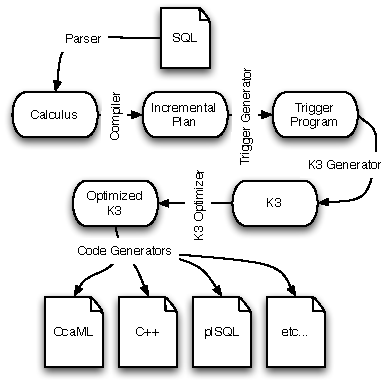
\includegraphics[width=3in]{CompilerFlow}


\section{Calculus}

\begin{verbatim}

type calc_type_t = 
  Int_Type | Double_Type | String_Type

type const_value_t = 
  Integer of int | Double of double | String of string

type var_t = string * calc_type_t

type value_t = 
  Var   of var_t
| Const of const_value_t

type cmp_t = Lt | Gt | Lte | Gte | Eq | Neq

type 'a calc_t =
  Sum        of calc_t list               (* c1 + c2 + ... *)
| Prod       of calc_t list               (* c1 * c2 * ... *)
| Neg        of calc_t                    (* -c *)
| Cmp        of value_t * cmp_t * value_t (* c1 [cmp] c2 *)
| AggSum     of var_t list * calc_t       (* AggSum([v1,v2,...], c) *)
| Value      of value_t                   (* Var(v) | Const(#) *)
| Relation   of string * var_t list       (* R(v1, v2, ...) *)
| External   of string * var_t list * 'a  (* {M1(v1, v2, ...) := 'a} *)
| Definition of var_t * calc_t            (* v <- c *)

type calculus_t = unit calc_t
\end{verbatim}

Most of the above is straightforward.  We parameterize the calc\_t type, because  the External type is, by definition outside of Calculus.  It is a reference to something outside, and we don't want Calculus to have to care about anything other than the API (a name and a set of parameters).  

Components using Calculus, conversely, need to be able to associate metadata with the External (i.e., initializers, etc...).  In particular, we would like to be able to associate invocations with the External, and we don't want Calculus to have any idea what an invocation is.  Parameterizing calc\_t is the cleanest way to accomplish this.

\section{Incremental Plan (IP)}


\begin{verbatim}

type schema_t = var_t list

type memo_t = 
    string                (* Name *)
    schema_t              (* Schema *)
  * calc_t                (* Defining calculus expression (the calculus 
                             expression that the memo is designed to 
                             maintain/compute *)
  * (   pm_t * string     (* Insert/Delete + Base Relation Name *)
      * map_op_t option   (* LHS initializer *)
      * map_op_t list     (* Update operations *)
    ) list

and map_op_t = (* += or := *)
    schema_t              (* LHS slice being updated/set *)
  * invocation_t          (* Invocation generating the slice *)

and invocation_t =
    calc_t                (* Calculus expression that the statement invokes *)
  * (                     (* Alternative ways of partitioning the invoked 
                             expression into different memos.  The head of this
                             list is the default approach. *)
      * calc_t            (* An expression over zero or more memos that is 
                             semantically equivalent to the invoked expression*)
      * list of memo_t    (* References to memos used by the above expression *)
    ) list

\end{verbatim}

\subsection{Assertions}
Assertions about the above memo and invocation types (the hypergraph):
\begin{itemize}
\item Initializers initialize the entire Memo, and therefore have no externally bound variables other than the invoked expression's input variables, and the variables which appear in the corresponding initializer.  If an input variable is not bound, it is a loop variable.

\item The access patterns that a Memo is required to support are defined by the set of bound variables in all of its incoming edges.

\item Initializers for memos on the RHS of an expression are stored as part of the calculus expression (External leaves) \footnote{Storing the whole initializer will make working with nonstandard maps (e.g., future work on range trees) difficult.  In effect, the External needs to store a reference to the entire process required to initialize a memo.  On the other hand, this initializer can and should be simplified/compiled given that the set of bound input variables will change.  A reasonable compromise might be to store a list of expressions that the initializer will need to evaluate}.  The LHS memo does not need to be initialized, since the output portion of the memo is guaranteed to be initialized and we'll never see a new input variable in a delta statement.

\item The root of an IP can be either a Memo or an Invocation.  The former corresponds to compiling a datastructure which continually maintains the exact query result.  The latter corresponds to compiling an executable which can efficiently (using incrementally maintained views) answer the posed query.

\end{itemize}

\begin{example}
The following image shows the incremental plan for the query:
$$Q = Sum([], R(a,b) * S(b,c) * T(c,d) * a * d)$$

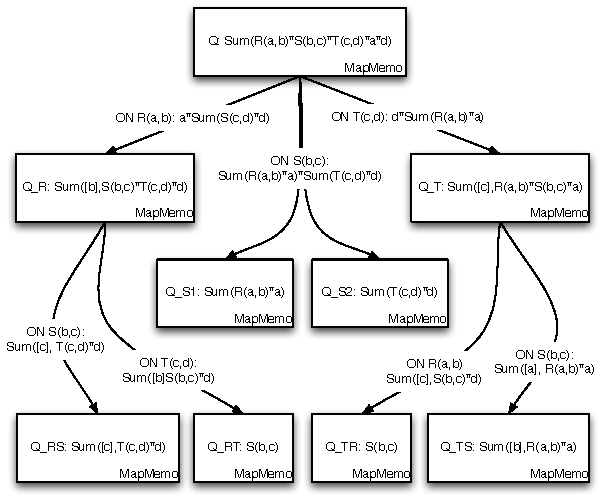
\includegraphics[width=5.0in]{IPExample}
\end{example}

\section{Compilation}

The goal of the compilation phase is to translate an arbitrary calculus expression into an Incremental Plan, as described above.  At an extremely high level, this process breaks down into a recursive loop over three steps: (1) {\bf Simplify} the expression, (2) {\bf Extract} portions of the expression for incremental maintenance, (3) Compute the {\bf delta} terms, and recurse for each.

To mirror the structure of the IP, make it possible to compile queries into both Memos and Invocations, and because step 1 in the above process produces a semantically equivalent query, the compiler is divided into two parts - {\bf compile\_memo} and {\bf compile\_invocation}.

\subsection{Calculus and Code}

Ultimately the goal of DBToaster is to produce code.  The structure of a calculus expression translates directly into how that expression will be evaluated.  Correspondingly, the compiler phase must be designed to ensure efficient code evaluation.  We now make several meaningful observations about calculus expressions and how they translate to the generated code.

\parsection{Input and Output Variables}
Variables appearing in a calculus expression take one of two forms: Input and Output.  Output variables appear on the LHS of definition terms or as part of a Relation term.  Given an expression, we can always identify its Output variables.  

Input variables appear in the expression as values, but are not bound within the expression (i.e., they are not Output variables).  Given an expression, we can always identify its Input variables.  Input variables can be thought of as {\it parameters} to the expression.

\parsection{Bags and Arities}
As a data parallel language, the fundamental datatype in calculus is the set (of tuples), or more precisely a bag.  Like a traditional bag, each tuple is associated with an arity, or number of times that the tuple appears in the bag.  Unlike traditional bags however, a tuple's arity can be negative, or even non-integral.  In this sense, the set is a map, the tuple is a key, and the arity is the corresponding value.  These two interpretations are mostly interchangeable.  

It is important to understand them both to understand how Calculus interacts with both the relational and aggregation aspects of SQL, and how to correctly interpret the {\tt Sum} and {\tt Prod} operators (discussed below).  The use of arity also explains why {\tt AggSum} acts as both a projection and an aggregation operator, since post-projection duplicates have their arities merged.

An important consequence is that in calculus, there is no distinction between $\{(\left<\ldots\right> = 0)\}$ and $\emptyset$.  That is, a tuple with arity 0 is not at all distinct from a tuple not present in a result set; Thus typically, when referring to the domain of an expression, we will consider only the elements of the set with arity $\neq 0$ \footnote{It should also be noted that while calculus does not make this distinction, later stages do; When storing a partially materialized result set, a zero arity indicates a tuple not present in the complete result set, while absence from the set indicates that the tuple's arity has not yet been computed.}

\parsection{Schemas and Singletons}
An expression's output variables correspond to the schema of all of its result tuples\footnote{{\tt Sum} can potentially be viewed as generating hybrid schemas, but like SQL's UNION we require that it operate only over subexpressions with identical schemas}.  The behavior of the {\tt Prod} operator in particular relates very closely to the schemas of its subexpressions -- in particular those with no output variables, termed {\it singletons}.  These are particularly important, because they have a finite domain at compile time (i.e., they do not require looping).  More on this later.

\parsection{Loops} 
Our current infrastructure focuses on single-threaded operation, so it is important to recognize that all calculus expressions represent an implicit loop over elements of the set of values produced by the expression.

If an expression appears nested inside a calculus operator, the calculus operator explicitly performs an operation over each element in the set (e.g., negation negates every element of the set).  

Even the top level expression can (and should) be interpreted as a loop; Whatever is evaluating the expression loops over each of its elements.  For example, the {\tt :=} and {\tt +=} operators loop over the entire domain, setting or incrementing the corresponding LHS map entry.

Note that there is a key difference between the traditional imperative notion of loops and the more set-oriented approach taken by calculus: the loop domain comes from within the loop block itself.  In terms of implementation each non-leaf, or operator term in calculus applies an operation to every element of the domain of its child expressions.  For unary operators (i.e., {\tt Neg} and {\tt AggSum}), the desired operation and imperative interpretation is clear; {\tt AggSum} for example, can be thought of as an inner loop.  The operator asserts that a particular subset of the loop domain is meaningful only within a specific subtree of the code.

N-ary operators (i.e., {\tt Prod} and {\tt Sum}) have a slightly different implementation interpretation.  Though Calculus is a primarily functional language, {\tt Sum} can be thought of as an imperative ``step," or operation in the loop.  From a set-loop-oriented perspective, one can think of this (roughly) as first iterating over the values on the left-hand side, and subsequently the right-hand.  Formally, the sum operator must merge duplicate values.  However, when converting a calculus expression to an imperative execution plan, it helps to think of each expression in the sum as an independent step in the loop.

\parsection{{\tt Prod} (and Singletons and Single-entry tables)}
If {\tt Sum} is an imperative step, then {\tt Prod} is more closely related to a continuation.  The intuition is that a calculus expression is parameterized (by input variables), and can influence control flow by returning a carefully selected set of results (e.g., a zero arity singleton to terminate the current loop iteration).  

A common instantiation of this behavior is via singleton expressions, which can affect the arity of tuples in the result set without affecting the domain: (1) {\tt Value} terms, (2) {\tt Cmp} terms, and (3) {\tt AggSum} terms with no group-by variables.

\begin{example}
Consider the following expression:
$$expr * (a \theta b)$$
This expression represents a simple filtering predicate: $(a \theta b)$.  More complex incremental predicates can be applied by using definition terms.  For example:
$${\tt AggSum}(expr_{in}.schema, expr_{in} * (a \gets expr_a) * (b \gets expr_b) * (a \theta b))$$
\end{example}

\parsection{{\tt Definition}}
Consider what happens if $expr_a$ and $expr_b$ are both singletons themselves.  Definition terms with singletons on the RHS do not affect the arity (they always evaluate to 1), nor do they affect the size of the tuple set (they always have a single value).  They do, however, extend the domain with additional variables (that can be used for filtering or further computation).  One way to think about this sort of behavior is as a continuation.

\parsection{Commutativity (and Associativity) of {\tt Prod}}
{\tt Prod} has some non-straightforward commutativity properties: Product is commutative {\bf unless} an Input variable appearing on the right hand side (i.e., a parameter) is present as an Output variable on the LHS \footnote{An exception to this rule occurs when there is a triple product with the variable in question being used as a parameter to the third subterm.  If the first and second subterms both output the variable in question, the third and second subterms commute, assuming no other conflicts occur.}.  In effect, a product term has a binding pattern, where variables are declared by their presence as output variables on the left, and used as input variables on the right.  As in programming languages, a variable's declaration must always precede its use.  

On a similar note, though {\tt Prod} is associative, the order of operations can impact the efficiency of evaluating the expression.  

\begin{example}
For example, consider the expression:
$${\tt AggSum}([c], f_1[][a] * f_2[][b] * f_3[a,b][c])$$
\end{example}

It is important to note that the variable $a$ does not affect evaluation of $f_2$.  Consequently, it might be more efficient to evaluate this expression as right-associative (especially if it is possible to curry $f_3$).  This process is analogous to join ordering.

\parsection{The (ir)relevance of {\tt AggSum}s}
Though it might appear otherwise, the role of {\tt AggSum}s is purely as a convenient annotation tool.  Without them, evaluating a calculus expression would require a repeated loop through the entire domain of the result set.  {\tt AggSum}s are based around the observation that the typical usage pattern of a calculus expression involves aggregating over subsets of the result domain.  Furthermore, certain variables only appear in parts of the expression and are not required as part of the output domain (i.e., we aggregate over them).  By wrapping the portions of the expression that use a particular variable in {\tt AggSum}s, we indicate that this subset of the overall loop domain is isolated to within the {AggSum} (and doing so, simplify code generation).

\subsection{Compiler Challenges}

\parsection{Extraction}
Given an arbitrary calculus expression, we can create a memo to persist and incrementally maintain its result set.  However, it is often inefficient to do so for the entire calculus expression.  

\begin{itemize}
\item The expression may consist of two or more independent sub-queries.  For example, the expression computes the numerical product of two (potentially group-by) aggregate queries.  Storing the full cross-product of all group-by terms involved is unnecessary. as the expression must iterate over each of them; its time complexity is the same regardless of whether the cross-product is materialized or generated at run-time.  Conversely, materializing the cross product generates unnecessary storage (and consequently maintenance) overhead. 
 
\item Portions of the expression may involve constants.  Applying the constant when the overall expression is evaluated does not increase the time complexity of doing so.  Moreover, the resultant memo is simpler and easier to re-use across multiple evaluations.

\item Similarly, the expression may contain parameters (i.e., Input Variables), either loose or within inequalities.  We can treat the parameters as constants (and perform any necessary filtering when the expression is evaluated), or fold them into the memo expression and create a caching memo.

\item Definition terms do not get simpler when their delta is taken.  Thus, for definitions that can not be eliminated (e.g., by variable unification), it is necessary to perform the definition computation at evaluation time.  
\end{itemize}

As a consequence, the compiler must include an extraction step, where it identifies portions of the expression that are to be represented as memos.  There are three components to this process (assuming that the expression has already been separated into monomials):

\begin{algorithmic}[1]
\STATE Constant and (if applicable) expressions involving input variables\todo{There are countless ways of defining ``expressions involving input variables''.  We should pick which (and how many) the compiler should use.} are pulled out of the expression and used solely in the invocation.
\STATE Definition terms are pulled out and ignored for the next step.
\STATE The expression is factorized into separate cross-product subexpressions. Each subexpression is replaced by a memo.
\STATE Definition terms are used in the memo, and we recurse over the expression that appears on the RHS of the definition term
\end{algorithmic}

\parsection{Variable Unification}
The input and output variables (both input and output, as well as their types) of a calculus expression can always be computed from the expression; external metadata is not required.  

Variable unification has an impact on the schema of an expression.  Not only can it potentially remove input and output variables, but it can turn input variables into output variables (i.e., if an input variable is unified with an output variable) \footnote{Of course, this poses some limitations with respect to extracted expressions.  The schema of a memo can not be changed after the fact.  Even if it is possible to perform further unification on a delta expression, the schema must be further adjusted to match the memo being updated.}

Variable unification itself takes two forms: (1) downward, and (2) upward.  

Upward unification is the harder of the two, because it requires knowledge of input variables.  A comparison between two variables $x = y$ can be unified upwards using one of the following two rules:
\begin{itemize}
\item $e := f(x) * (x = y)$ becomes $(x \gets y) * f(x)$ iff $x$ is not already defined in the evaluation environment \footnote{note that it is not just an assertion that $x$ is not an input variable; $x$ can not be bound anywhere to the left of $e$, even if it is present as an output variable in $f(x)$.}.
\item $e := f(y) * (x = y)$ becomes $(y \gets x) * f(y)$ iff $y$ is not already defined in the evaluation environment.
\end{itemize}

Simpler, is downward unification.  An expression of the form:
$${\tt AggSum}\left([dom(f(x)) - \{x\}], (x \gets y) * f(x)\right)$$
can be unified down to $f(y)$.  Critically, note that this process is reversible.  Given a variable $x$ with a name not defined in the environment or domain of expression $e$ (and just to be safe, not used in the expression either), we can transform $g()$ into
$${\tt AggSum}\left([dom(g())], (x \gets \{anything\}) * g()\right)$$
Here, $\{anything\}$ can in fact be replaced by anything with an empty input and output domain.

In particular, this allows us to perform factorization over variable definitions.  For example
$${\tt AggSum}\left([dom(f(x)) - x], (x \gets y) * f(x)\right) + g()$$
$${\tt AggSum}\left([dom(f(x)) - x], (x \gets y) * f(x)\right) + {\tt AggSum}\left([dom(g())], (x \gets y) * g()\right)$$
$${\tt AggSum}\left([dom(f(x)) - x], ((x \gets y) * f(x)) + ((x \gets y) * g()) \right)$$
$${\tt AggSum}\left([dom(f(x)) - x], (x \gets y) * (f(x) + g()) \right)$$

In other words, we can lift definition terms as far up through summation terms as we like, as long as there are no variable naming conflicts in the terms we distribute across.  Once a definition term is at the very top, we can perform downward unification as desired.


\subsection{Algorithms}

\parsection{compile\_memo (Standard Map)}

This is the first of two mutually recursive steps in (and entry points into) the compilation process.  

\begin{algorithmic}
\REQUIRE{calc\_t $definition$, schema\_t $schema$}
\ENSURE{A memo\_t $memo$}
\STATE Generate a unique name for $memo$
\STATE {\bf calc\_simplify}($definition$)
\STATE $memo.definition \gets definition$
\FORALL{(Reln,Delta) $(rel, d\_defn) \in$ compute\_deltas($definition$)}
  \STATE {\bf calc\_simplify}($d\_defn$)
  \STATE $memo.deltas[rel].update \gets$ {\bf compile\_invocation}($d\_defn$)
\ENDFOR
\FORALL{Reln $rel \in$ $definition$}
  \STATE $relinit \gets$ {\bf initializer\_for\_memo}($memo$)
  \STATE Substituting $rel$'s variables into $relinit$ (or all of them)
  \STATE {\bf calc\_simplify}($relinit$)
  \STATE $memo.deltas[rel].init \gets$ {\bf compile\_invocation}($relinit$)
\ENDFOR
\end{algorithmic}




\parsection{compile\_invocation}
\begin{algorithmic}
\REQUIRE{A calc\_t $expression$}
\ENSURE{An invocation\_t $invocation$}
\STATE Separate the monomial into independent monomial components (i.e., monomials with no overlapping internally-bound variables)
\FORALL{Independent calc\_t component $c \in expression$}
  \STATE Pull out all remaining definition terms and create a memo for their RHS.  Then, if any of the remaining terms contain a relation term...
  \STATE (Optimization Choice B1: More read work): Pull out all comparison terms with an input variable and create a memo for the remaining terms.
  \STATE (Optimization Choice B2: More write work + Bigger memos): Create a memo for all the remaining terms.
  \FORALL{Memo expression $m\_expr \in c$}
    \STATE $memo \gets$ {\bf compile\_memo}($m\_expr$)
    \STATE $init \gets$ {\bf initializer\_for\_memo($memo$)}
    \STATE {\bf calc\_simplify}($init$)
    \STATE {\bf compile\_invocation}($init$)
    \STATE Replace the corresponding terms in $c$ with $External(memo, \ldots, init)$
  \ENDFOR
\ENDFOR
\STATE Rejoin the components into a polynomial expression.
\end{algorithmic}

\parsection{initializer\_for\_memo}
\begin{algorithmic}
\REQUIRE{A memo\_t $memo$ with compiled triggers}
\ENSURE{An calc\_t to initialize $memo$ if necessary}
\IF{$definition$ has unbound variables}
  \STATE (Optimization Choice A1: Bottom Up): Generate an initialization expression $init$ by taking a delta invocation (pick one, or generate them all), multiplying it by the delta relation.
  \STATE (Optimization Choice A2: Top Down): Generate an initialization expression $init$ by taking $definition$.  Note that when calling {\bf compile\_invocation}, this option will go into an infinite loop with optimization choice B2.
  \STATE (Optimization Choice A3: No opt): Generate an initialization invocation by replacing relations in $definition$ with memos.  Requires a special {\bf compile\_invocation}.
  \STATE Replace variables in the initializer with the corresponding variables in $schema$.
  \STATE {\bf return} $init$
\ELSE
  \STATE {\bf return} $none$
\ENDIF
\end{algorithmic}

\parsection{calc\_simplify}
\begin{algorithmic}
\REQUIRE{calc\_t $expression$, a set of externally bound var\_t $ivars$}
\ENSURE{A calc\_t Sum() of $monomials$}
\STATE Pull sums in $expression$ up to the top, generating a list of $monomials$
\FORALL{$m \in monomials$}
  \REPEAT
    \STATE {\bf calc\_unify\_vars}($m$)
    \STATE Flatten products
    \STATE Pull AggSums up and merge where possible
    \STATE Push negation down and merge where possible
    \STATE Move constants left and merge where possible
    \STATE Move comparisons right
    \STATE Eliminate $m$ if it has a 0 or a contradiction (e.g., $(a \theta b) * (a \bar \theta b)$, $(a \neq a)$, $(a < a)$, \ldots)
    \STATE \COMMENT{Some sort of ``lexical" sort might be appropriate}
  \UNTIL{fixedpoint($m$)}
  \STATE Cancel negated sums (e.g., $a + (- a)$)
  \STATE Recurse over subterms of definition terms
\ENDFOR
\STATE 
\end{algorithmic}

\parsection{calc\_unify\_vars}
\begin{algorithmic}
\REQUIRE{a monomial calc\_t $expression$}
\ENSURE{$expression$ with variables unified}
\FORALL{Definition $(v \leftarrow c) \in$ the root level of $expression$}
  \IF{$c$ is a variable bound earlier in the expression, or a constant}
    \STATE replace all occurrences of $v$ in $expression$ with $c$
    \STATE remove the definition ($v \leftarrow c$) from $expression$
  \ENDIF
  \STATE replace all loose (i.e., not in comparison, external, or relation terms) occurrences of $v$ with $c$.
  \IF{$v$ no longer appears in $expression$, or in its parent $AggSum$}
    \STATE remove the definition ($v \leftarrow c$) from $expression$
  \ENDIF
\ENDFOR
\FORALL{Equality Comparison w/ Const $(v = c) \in expression$}
  \STATE Replace $v$ in the expression with $c$
  \STATE remove the comparison ($v = c$) from $expression$
\ENDFOR
\FORALL{Equality Comparison w/ Var $(v_1 = v_2) \in expression$}
  \STATE If possible, replace $v_1$ in the expression with $v_2$ or visa versa
  \STATE remove the comparison ($v_1 = v_2$) from $expression$
\ENDFOR
\end{algorithmic}

\parsection{compute\_deltas}
\begin{algorithmic}
\REQUIRE{A calc\_t $expression$}
\ENSURE{An associative list of relation to calc\_t pairs}
\STATE {\bf calc\_simplify}($expression$)
\FORALL{Monomial calc\_t $m \in expression$}
  \FORALL{Relation $r \in m$}
    \STATE Gather $(r \rightarrow {\bf calc\_simplify}({\bf generate\_delta}(m, r)))$
  \ENDFOR
\ENDFOR
\end{algorithmic}

\parsection{generate\_delta}
\begin{algorithmic}
\REQUIRE{A simplified calc\_t $expression$, A relation $r(r_1,r_2,\ldots)$}
\ENSURE{A calc\_t delta expression}
\IF{$m$ is a {\tt Prod[$m_1$]}}
  \STATE {\bf return} {${\bf generate\_delta}(m_1)$}
\ELSIF{$m$ is a {\tt Prod[$m_1, m_2, \ldots$]}}
  \STATE {\bf return} {\tt Sum[Prod[{\bf generate\_delta}($m_1$),$m_2,\ldots$], \\
  \hspace*{1in}Prod[$m_1$,{\bf generate\_delta}(Prod[$m_2,\ldots$])], \\
  \hspace*{1in}Prod[{\bf generate\_delta}($m_1$), {\bf generate\_delta}(Prod[$m_2,\ldots$])]]}
\ELSIF{$m$ is a {\tt Neg($m_1$)}}
  \STATE {\bf return} {\tt Neg({\bf generate\_delta}($m_1$))}
\ELSIF{$m$ is a {\tt AggSum($\ldots, m_1$)}}
  \STATE {\bf return} {\tt AggSum($\ldots, m_1$)}
\ELSIF{$m$ is a {\tt Value($\ldots$)}}
  \STATE {\bf return} $\emptyset$
\ELSIF{$m$ is a Relation($r$, $v_1,v_2,\ldots$)}
  \STATE {\bf return} {\tt Prod[($v_1 \leftarrow r_1$), ($v_2 \leftarrow r_2$), \ldots]}
\ELSIF{$m$ is a Relation(\ldots)}
  \STATE {\bf return} $\emptyset$
\ELSIF{$m$ is an External}
  \STATE {\bf ERROR} \COMMENT{or work off of the external initializer}
\ELSIF{$m$ is a {\tt Definition($v,m_1$)}}
  \STATE {\bf return} {\tt Definition($v,m_1+{\bf generate\_delta}(m_1)$) - Definition($v,m_1$)}
\ELSIF{$m$ is a {\tt Cmp(\ldots)}}
  \STATE {\bf return} $\emptyset$
\ENDIF

\end{algorithmic}

\section{Trigger Generation}

The triggers\_for\_X functions translate an Incremental Plan into a set of triggers.  Each trigger is of the form: (1) The Event/Relation name (Variables appearing in the event/relation are drawn from the database schema).  (2) The set of initializers that need to be invoked if necessary (with variables bound as per the schema).  (3) The set of update operations that need to be invoked (with variables bound as per the schema).

\begin{verbatim}
let trigger_t = 
    string * var_t list                 (* Relation Schema *)
                                        (* Maybe make it a (string * (...))
                                           to make it into an assoc list *)
  * (string * var_t list * calc_t)      (* LHS Initializer *)
  * (string * var_t list * calc_t) list (* Updates *)
\end{verbatim}

\parsection{triggers\_for\_memo}
\begin{algorithmic}
\REQUIRE{memo\_t $memo$}
\ENSURE{A trigger\_t of initializers and triggers, and a list of memos}
\FORALL{Event $e \in memo$}
  \STATE $(impl,statements,prog) \gets$ \textbf{triggers\_for\_invocation}($e.initializer.expression$)
  \STATE Gather $statements$ and $prog$
  \STATE Add initiailzer ($memo.name$, $e.initializer.vars$, $impl$)
  \FORALL{Invocation $i \in e.updates$}
    \STATE $(impl,statements,prog) \gets$ \textbf{triggers\_for\_invocation}($i.expression$)
    \STATE Gather $statements$ and $prog$
    \STATE Add update ($memo.name$, $i.vars$, $impl$)
  \ENDFOR
\ENDFOR
\STATE \textbf{return} The gathered trigger\_ts and memo\_t list
\end{algorithmic}

\parsection{triggers\_for\_invocation}
\begin{algorithmic}
\REQUIRE{invocation\_t $invoc$}
\ENSURE{A calc\_t and a trigger\_t and prog\_t}
\STATE Select an implementation $impl \in invoc$
\FORALL{Memo $m \in impl$}
  \STATE Gather \textbf{triggers\_for\_memo}(m)
\ENDFOR
\STATE {\bf return} $impl$ and the gathered trigger\_t and memo\_t list
\end{algorithmic}

\subsection{Commentary}
We refer to triggers\_for\_invocation's second parameter as its context.  Context is a way of passing variable bindings through multiple layers of triggers\_for\_invocation, and can contain two types of bindings: (1) Input variables can be bound from above (i.e., as event variables), and (2) Input variables can be bound from the side (i.e., from another map).  

Case 2 only occurs if we have multi-level initializers (i.e., if the initializer for a map reads from a map with an initializer).  In our current design, this is not possible.  Consequently, the algorithm above only handles Case 1.  In order to support Case 2, the following would need to happen:
\begin{itemize}
\item The context needs to be extended to be able to express actual domains (e.g., It needs to be able to express "variables $b$ and $c$ in $M_1[][a,b,c]$").
\item The generated initializer needs to have a way of iterating over the corresponding domain.  This can either be done by applying the above extensions to the datastructure, or by adding in a domain loop like 
$$M_1[a,b][] :=  (dummy \leftarrow M_2[a]) * TheRestOfTheInitializer$$
The former would be preferable, as the latter produces a calculus expression where the input variable is bound from below.
\end{itemize}


\end{document}  